\documentclass[acmnow]{acmtrans2m}
\usepackage{amssymb}
\usepackage{amscd}
\usepackage{amsmath}
\usepackage[dvipdfm]{graphicx}
\usepackage{color}

\newtheorem{theorem}{Theorem}[section]
\newtheorem{conjecture}[theorem]{Conjecture}
\newtheorem{corollary}[theorem]{Corollary}
\newtheorem{proposition}[theorem]{Proposition}
\newtheorem{lemma}[theorem]{Lemma}
\newdef{definition}[theorem]{Definition}
\newdef{remark}[theorem]{Remark}

\def\F2{{\mathbb F}_2}
\def\wt{{\rm wt}}
\def\wo{{\rm wt}_o}
\def\wf{{\rm wt}_f}
\def\UL{{\rm ul}}
\def\bx{{{\mathbf x}}}
\def\by{{{\mathbf y}}}
\def\bz{{{\mathbf z}}}
\def\bw{{{\mathbf w}}}
\def\bu{{{\mathbf u}}}

\def\im{{\mathrm{Im}}}
\def\ker{{\mathrm{Ker}}}
\def\id{{\mathrm{Id}}}
\def\tr{{\mathrm{tr}}}

\title{SIMD-oriented Fast Mersenne Twister:
a 128-bit Pseudorandom Number Generator
}
            
\author{Mutsuo Saito and Makoto Matsumoto, Hiroshima University \\
}
            
\begin{abstract} 
Mersenne Twister (MT)
is a widely-used fast pseudorandom number generator (PRNG)
with a long period of $2^{19937}-1$,
designed 10 years ago based on 32-bit operations.
In this decade, CPUs for personal computers
acquired new features, such as 
Single Instruction Multiple Data (SIMD) operations
(i.e., 128-bit operations) and multi-stage pipelines.
Here we propose a 128-bit based 
PRNG, named SIMD-oriented Fast Mersenne Twister
(SFMT), which is analogous to MT but making full use
of these features. Its recursion fits to the pipeline processing
better than MT, and it is roughly twice faster than 
optimized MT using SIMD operations.
Moreover, the dimension of equidistibution of SFMT, 
as a 32-bit integer generator,
is better than MT. 

We also introduce 
a block-generation function, 
which fills an array of 32-bit integers at one time.
It speeds up the generation by a factor of two. 
A speed comparison with other modern generators, 
such as multiplicative recursive generators,
shows an advantage of SFMT.
\end{abstract}
            
\category{G.3}{Mathematics of Computing}{PROBABILITY AND STATISTICS}[Random number generation]

\terms{Algorithms, Theory} 
            
\keywords{
Mersenne Twister,
SFMT, 
SIMD, 
128-bit,
block generation
}

\begin{document}
\maketitle

\begin{bottomstuff}
Authors' addresses: 
M. Saito and M. Matsumoto: Department of Mathematics, Hiroshima University,
Kagamiyama 1-3-1, Higashi-Hiroshima, Hiroshima 739-8526, Japan;
email: \{saito, m-mat\}@math.sci.hiroshima-u.ac.jp;

This study is partially supported by JSPS/Ministry of Education
Grant-in-Aid for Scientific Research No.18654021, No. 16204002,
and JSPS Core-to-Core Program No.18005.
\end{bottomstuff}

\section{Introduction}
Recently, the scale of simulations is getting larger,
and faster pseudorandom number generators (PRNGs)
are required. The power of CPUs for
usual personal computers are now sufficiently strong
for such purposes, and the necessity of efficient PRNGs 
for CPUs on PC is increasing.
One of such generators is Mersenne Twister (MT) \cite{MT},
which is based on a linear recursion modulo 2 over 32-bit
integers. An implementation MT19937 has 
the period of $2^{19937}-1$ and 
can generate
roughly $10^8$ 32-bit pseudorandom integers per a second.

MT was designed 10 years ago,
and the architectures of CPUs for Personal Computers,
such as Pentium and PowerPC, has been changed.
They have
Single Instruction Multiple Data (SIMD) operations,
which may be regarded as operations 
on 128-bit registers. Also, they have more registers
and automatic parallelisms by multi-stage pipelining. 
These are not reflected in the design of MT. 

In this article, we propose a MT-like 
pseudorandom number generator
that makes full use of these new features: SFMT, 
SIMD-oriented Mersenne Twister. 
We implemented an SFMT with period a multiple of $2^{19937}-1$, named
SFMT19937,
which has a better equidistribution property than MT. 
SFMT is much faster than MT, even without using SIMD instructions. 

There is an argument that the CPU time consumed for 
function call to PRNG routine occupies large part of
the random number generation, and consequently 
it is not so important to improve the speed of PRNG 
(cf. \cite{XORSHIFT}).
This is not always the case: 
one can avoid the function calls by (1) inline-expansion
and/or (2) generation of pseudorandom numbers in an array
at one call. Actually some demanding users re-coded MT to avoid the 
function call, see the homepage of \cite{MT}. 
In this article, we introduce a block-generation scheme, which 
is much faster than using function calls.

\section{SIMD-oriented Fast Mersenne Twister}\label{sec:jump}

We propose SIMD-oriented Fast Mersenne Twister (SFMT) 
pseudorandom number generator. It is a
linear feedbacked shift register generator based
on a recursion over $\F2^{128}$.
We identify
the set of bit $\{0,1\}$
with the two element field $\F2$. This means that
every arithmetic operation is done modulo 2. 
A $w$-bit integer is identified with 
a horizontal vector in $\F2^{w}$, and 
$+$ denotes the sum as vectors (i.e., 
bit-wise exor), not as integers.
We consider three cases: $w$ is 32, 64 or 128.

\subsection{LFSR generators}
A Linear Feedbacked 
Shift Register (LFSR) method is to generate
a sequence $\bx_0, \bx_1, \bx_2, \ldots$
of elements $\F2^{w}$ by a recursion
\begin{equation}\label{eq:recursion}
\bx_{i+N}:=g(\bx_i, \bx_{i+1}, \ldots, \bx_{i+N-1}),
\end{equation}
where $\bx_i \in \F2^{w}$ and 
$g:(\F2^{w})^N \to \F2^{w}$ is an $\F2$-linear function
(i.e., the multiplication of a $(wN \times w)$-matrix 
from the right to a $wN$-dimensional vector)
and use it as a pseudorandom $w$-bit integer sequence.
In the implementation, this recursion is computed
by using an array {\tt W[0..N-1]} of $N$ integers of $w$-bit size,
by the simultaneous substitutions
$$
{\tt
W[0] \leftarrow W[1],\ 
W[1] \leftarrow W[2],\  \ldots,
W[N-2] \leftarrow W[N-1],\  
W[N-1] \leftarrow} g({\tt W[0]},\ldots,{\tt W[N-1]}). 
$$
The first $N-1$ substitutions shift the content of 
the array, hence the name of LFSR. 
Note that in the implementation we may use 
an indexing technique to avoid
computing these substitutions, see \cite[P.28 Algorithm A]{knuth:bible}.
The array {\tt W[0..N-1]} is called the state array.
Before starting the generation, we need to 
set some values to the state array, 
which is called the initial state. 

Mersenne Twister (MT) \cite{MT}
is an example with
$$
g(\bw_0,\ldots,\bw_{N-1})=(\bw_0|\bw_1)A + \bw_M,
$$
where $(\bw_0|\bw_1)$ denotes
the concatenation of 
$32-r$ MSBs of $\bw_0$ and $r$ LSBs of $\bw_1$,
and $A$ is a $(32\times 32)$-matrix 
for which the multiplication $\bw A$ is computable 
by a few bit-operations.
Its period is $2^{32N-r}-1$, chosen to be a Mersenne prime.
To obtain better equidistribution property, 
MT transforms the sequence by
a suitably chosen $(32\times 32)$ matrix $T$,
by outputting
$\bx_0T , \bx_1T, \bx_2T, \ldots$
(called tempering).

\subsection{New features of modern CPUs for personal computers.}
Modern CPUs for personal computers (e.g.\ Pentium and
PowerPC) have new features such as 
(1) fast integer multiplication instructions
(2) fast floating point operations 
(3) SIMD operations 
(4) multi-stage pipelining.
These were not available 
for standard CPUs for PC, when MT was designed.

An advantage of $\F2$-linear generators 
over integer multiplication generators 
(such as Linear Congruential Generators \cite{knuth:bible}
or Multiple Recursive Generators \cite{MRG})
was high-speed generation by avoiding multiplications.
This advantage is now smaller, since 
32-bit integer multiplication is quite fast. 

Among the new features,
(3) and (4) fit to $\F2$-linear generators. 
Our idea is simple: to design
a 128-bit integer PRNG, considering
the benefit of such parallelism in the recursion.

\subsection{The recursion of SFMT}
We choose $g$ in the recursion (\ref{eq:recursion}) as
\begin{eqnarray}\label{eq:rec-SFMT}
g(\bw_0,\ldots,\bw_{N-1}) 
%&=& g(\bw_0, \bw_M, \bw_{N-2}, \bw_{N-1}) \\
&=& \bw_0A + \bw_MB + \bw_{N-2}C + \bw_{N-1}D,
\end{eqnarray}
% \[x_{n+i} = x_{n-1+i}A + x_{n-2+i}B+ x_{m+i}C + x_{i}D,\]
where 
$\bw_0, \bw_M, \ldots$ are $w(=128)$-bit integers 
(= horizontal vectors in $\F2^{128}$),
and $A, B, C, D$ are sparse $128 \times 128$ matrices
over $\F2$ for which 
$\bw A, \bw B, \bw C, \bw D$ can be computed by
a few SIMD bit-operations.
%\begin{figure}
%\begin{center}
%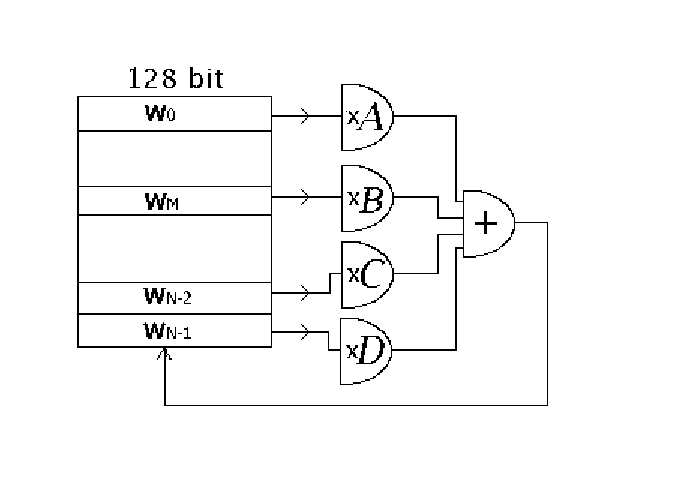
\includegraphics[width=0.7\linewidth]{sfmt-a.eps}
%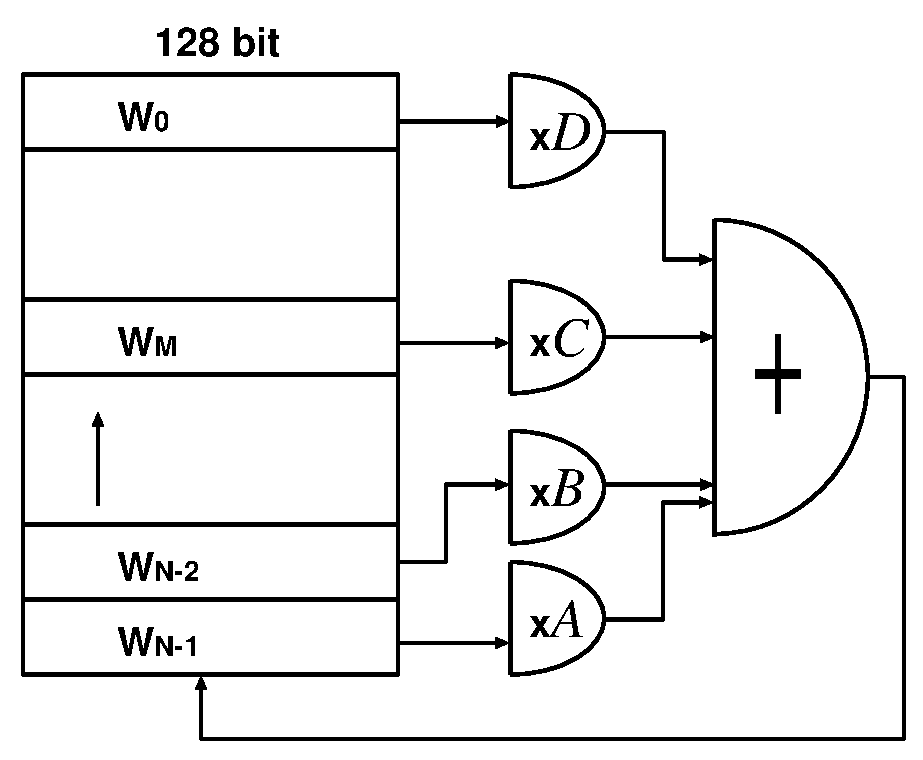
\includegraphics[width=0.7\linewidth]{sfmt-a2.eps}
%\end{center}
%\caption{The transition function of SIMD-oriented Fast MT.}
%\end{figure}
The choice of the suffixes $N-1$, $N-2$ is for the 
speed. In the implementation of $g$, 
{\tt W[0]} and {\tt W[M]} are read from the array
{\tt W}, while the copies of 
{\tt W[N-2]} and {\tt W[N-1]}
are kept in 
two 128-bit registers in the CPU, 
say {\tt r1} and {\tt r2}. Concretely saying, we assign 
${\tt r2} \leftarrow {\tt r1}$ and
${\tt r1} \leftarrow \mbox{``the result of (\ref{eq:rec-SFMT})''}$
at every generation, then {\tt r2} ({\tt r1}) keeps
a copy of {\tt W[N-2]} ({\tt W[N-1]}, respectively). 
The merit of doing this is to use pipeline effectively. To fetch 
{\tt W[0]} and {\tt W[M]} from the memory takes some
time. In the meanwhile, 
CPU can compute $\bw_{N-2}C$ and $\bw_{N-1}D$,
because copies of $\bw_{N-2}$ and $\bw_{N-1}$ are kept 
in the registers. This selection was made through experiments
on the speed of generation.

By trial and error, 
we searched for a set of parameters of SFMT,
with period being a multiple of $2^{19937}-1$
and good equidistribution property.
The degree of recursion $N$ is $\lceil 19937/128 \rceil=156$, 
and the linear transformations $A,B,C,D$ are as follows.
\begin{itemize}
\item 
$\bw A := (\bw \stackrel{128}{<<} 8) + \bw.$

This notation means that $\bw$ is regarded
as a single 128-bit integer, and 
$\bw A$ is the result of the left-shift
of $\bw$ by 8 bits. There is such a SIMD operation
in both Pentium SSE2 and PowerPC AltiVec SIMD instruction 
sets (SSE2 permits only a multiple of 8
as the amount of shifting). 
Note that the notation $+$ means the exclusive-or
in this article.

\item
$\bw B := (\bw \stackrel{32}{>>} 11) \& (\mbox{\tt BFFFFFF6 BFFAFFFF DDFECB7F DFFFFFEF}).$

This notation means that $\bw$ is considered to be 
a quadruple of $32$-bit integers, and
each $32$-bit integer is shifted to the right by 11 bit,
(thus the most significant bit is filled with 0s, 
for each 32-bit integers).
The C-like notation $\&$ means the bitwise AND
with a constant 128-bit integer,
denoted in the hexadecimal form
(MSB is at the left). 

In the search,
this constant is randomly generated as follows. 
Each bit in the 128-bit integer is independently 
randomly chosen, with the probability to choose 1 being $7/8$.
This is because we prefer to have more 1's for a denser 
feedback.

\item 
$\bw C := (\bw \stackrel{128}{>>} 8).$

The notation 
$(\bw \stackrel{128}{>>} 8)$ is the 128-bitwise right shift 
by 8 bits, as above.

\item
$\bw D := (\bw \stackrel{32}{<<} 18).$

Similarly to the above,
$\bw$ is cut into four pieces of 32-bit integers,
and each of them is shifted by 18 bits to the left.
\end{itemize}
All these instructions are available in 
both Intel Pentium's SSE2 and PowerPC's AltiVec SIMD instruction sets.
Figure~\ref{fig:SFMT-B2} shows a concrete description
of SFMT19937 generator with period $2^{19937}-1$.
\begin{figure}
\begin{center}
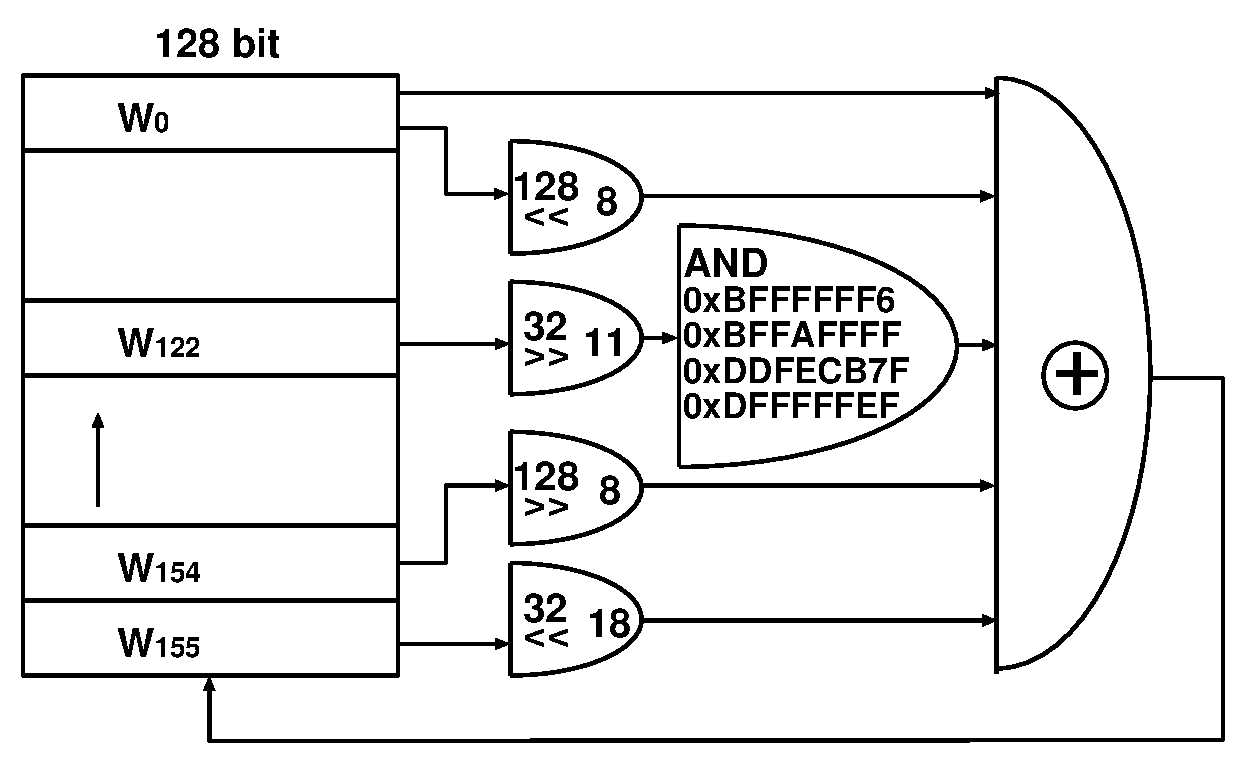
\includegraphics[width=0.7\linewidth]{sfmt-b2.eps}
\end{center}
\caption{A circuit-like description of SFMT19937.}
\label{fig:SFMT-B2}
\end{figure}

\subsection{How we selected the recursion and parameters.}
In typical applications, we need 32-bit integers 
or 64-bit integers as the output of PRNGs, instead of 
128-bit integers.
SFMT19937 is a 128-bit integer generator, but 
we may regard it as a 32-bit (64-bit) integer generator, by
partitioning each 128-bit into four 32-bit (two 64-bit, respectively)
integers. 
Let $\bx$ be a 128-bit integer. Then we denote
by 
$\bx[0]$ the 32 LSBs of $\bx$, 
$\bx[1]$ the 33rd--64th bits,
$\bx[2]$ the 65rd--96th bits,
and $\bx[3]$ the 32 MSBs. Thus, $\bx$ is
the concatenation of 
$\bx[3], \bx[2], \bx[1], \bx[0]$, in this order.

SFMT generates a sequence
$\bx_0, \bx_1, \bx_2, \ldots$ of 128-bit integers. 
Then, they are converted to a sequence of 32-bit integers
$\bx_0[0], \bx_0[1], \bx_0[2], \bx_0[3], \bx_1[0], \bx_1[1],\ldots$,
or 64-bit integers
$\bx_0[1]\bx_0[0], \bx_0[3]\bx_0[2], \bx_1[1]\bx_1[0]$,
i.e., by the so-called little-endian system 
(see \S\ref{sec:portability} for a compatible implementation
 with big-endian systems).

We write codes to compute (the lower bounds of) the period
(see \S\ref{sec:period}),
the dimension of equidistribution (DE, see below),
and to measure the generation speed for Pentium SSE2
and PowerPC AltiVec, with and without SIMD, as 32-bit 
or 64-bit integer generators. 

We fixed a type of recursion,
then using a small model (e.g. the period is a smaller
Mersenne prime $2^{607}-1$), we tested whether it
attains the desired period, good DE, and fast generations,
by trial and error on the type of recursion, 
and reached (\ref{eq:rec-SFMT}).
Then, we searched for the parameters 
with period being a nonzero multiple of $2^{19937}-1$. 
Roughly 10 sets of parameters are found per a day,
by using four AMD Athlon 64 machines. 
We selected the best parameter with respect to DE.

We briefly recall the definition of dimension of 
equidistribution (cf. \cite{CLT}). 
\begin{definition}\label{def:DE}
A periodic sequence with period $P$
$$\chi:=\bx_0, \bx_1, \ldots, \bx_{P-1}, \bx_P=\bx_0, \ldots$$
of $v$-bit integers is said to be {\em $k$-dimensionally equidistributed}
if any $kv$-bit pattern occurs equally often as a $k$-tuple
$$
(\bx_i, \bx_{i+1}, \ldots, \bx_{i+k-1})
$$
for a period $i=0,\ldots, P-1$.
We allow an exception for 
the all-zero pattern, which may occur once less often.
(This last loosening of the condition is technically
necessary, because the zero state does not occur
in an $\F2$-linear generator). 
The largest value of such $k$ is called the dimension 
of equidistribution (DE).
\end{definition}

We want to generalise this definition slightly.
We define the $k$-window set of the periodic sequence $\chi$
as
$$
W_k(\chi):=
\{(\bx_i, \bx_{i+1}, \ldots, \bx_{i+k-1}) | 
i =0,1,\ldots, P-1\},
$$
which is considered as a {\em multi-set}, namely, 
the multiplicity of each element is considered. 

For a positive integer $m$ and a multi-set $T$,
let us denote by $m \cdot T$ the multi-set 
where the multiplicity of each element in $T$ is
multiplied by $m$. Then, the above definition of
equidistribution is equivalent to 
$$
W_k(\chi)=(m\cdot O^k) \setminus \{{\mathbf 0}\},
$$
where $m$ is the multiplicity of the occurrences,
and the operator $\setminus$ means that the multiplicity
of ${\mathbf 0}$ is subtracted by one. 

\begin{definition}
In the above setting, if there exist a positive integer $m$ 
and a multi-subset
$D \subset (m\cdot O^k)$
such that
$$
W_k(\chi)=(m\cdot O^k) \setminus D,
$$
we say that $\chi$ is $k$-dimensionally equidistributed 
with defect ratio $\#(D)/\#(m \cdot O^k)$, 
where the cardinality is counted with multiplicity. 
\end{definition}
Thus, in Definition~\ref{def:DE}, the defect ratio upto $1/(P+1)$
is allowed to claim the dimension of equidistribution.
If $P=2^{19937}-1$, then $1/(P+1)=2^{-19937}$. 
In the following, the dimension of equidistribution 
allows the defect ratio upto $2^{-19937}$. 

For a $w$-bit integer sequence, its {\em dimension of 
equidistribution at $v$-bit accuracy} $k(v)$
is defined as the DE of the $v$-bit sequence, obtained by extracting
the $v$ MSBs from each of $w$-bit integers.
If the defect ratio is $1/(P+1)$, 
then there is an upper bound 
$$
k(v) \leq \lfloor \log_2 (P+1) / v \rfloor.
$$
The gap between the realized $k(v)$ and the upperbound is
called the dimension defect at $v$ of the sequence,
and denoted by
$$
d(v):=\lfloor \log_2 (P+1) / v \rfloor -k(v).
$$
The summation of all the dimension defects at
$1 \leq v \leq 32$ is called the total dimension defect, 
denoted by $\Delta$.

There is a difficulty in computing $k(v)$ when 
a 128-bit integer generator is used as a 32-bit 
(or 64-bit) integer generator.
We solved this by using weighted lattice method,
generalising \cite{CLT}. Since the algorithm involves
rather complicated mathematics, we omit it here
(we plan another article for this). 

The algorithm gives a (rather tight) 
lower bound $k'(v)$ of $k(v)$ for each $v$, 
and $k'(v) \leq \lceil 19937/v \rceil$ holds
for SFMT19937.
Consequently, we redefine the dimension defect for SFMT19937 by
$$
d(v):=\lceil 19937/v \rceil - k'(v) 
\mbox{ and } \Delta:=\sum_{v=1}^w d(v).
$$
The meaning of $k'(v)$ and a justification for this 
definition will be explained in the planned article.

\section{Comparison of the speed}\label{sec:comp-speed}
We compared two algorithms: MT19937 and SFMT19937,
with implementations with and without SIMD instructions.

We measured the speeds for four different CPUs:
Pentium M 1.4GHz, Pentium IV 3GHz, 
AMD Athlon 64 3800+, and PowerPC G4 1.33GHz.  
In returning the random values, we use two different ways.
One is the sequential generation, where one 32-bit random 
integer is returned for one call. 
The other is the block generation, where an array
of random integers is generated for one call (for 
detail, see \S\ref{sec:block} below). 

We measured the consumed CPU time in second, 
for $10^8$ generations of 32-bit integers. More precisely,
in the block generation case, we generate $10^5$
of 32-bit random integers by one call, and it is iterated
for $10^3$ times. 
In the sequential generation case, the same $10^8$
of 32-bit integers are generated, one per a call.
To avoid the function call, the code uses 
inline declaration. 
More precisely: we used the inline declaration
{\tt inline}
and unsigned 32-bit, 64-bit integer types 
{\tt uint32\_t}, {\tt uint64\_t} defined in 
INTERNATIONAL STANDARD ISO/IEC 9899 : 1999(E) 
Programming Language-C, Second Edition
(which we shall refer to as C99 in the rest of this article).
Implementations without SIMD are written in C99,
whereas those with SIMD use
some standard SIMD extension of C99 supported by 
the compilers icl (Intel C compiler) and gcc.

Table~\ref{tab:speed} summarises the comparison of 
the speed. The first four lines list the CPU-time
(in second) needed to generate $10^8$ of
32-bit integers, for Pentium-M CPU with Intel C/C++
compiler. The first line lists the seconds for
block-generation scheme. The second line shows the 
ratio of the CPU-time to that of 
SFMT(SIMD). Thus, SFMT coded in SIMD is 1.94 times
faster than MT coded in SIMD, and 3.53 times faster
than MT without SIMD. The third line lists the seconds
for sequential generation scheme. The fourth line
lists the ratio of them, with the basis taken
at SFMT(SIMD) block-generation (not sequential). 
Thus, the block-generation of SFMT(SIMD) is 2.78 times
faster than the sequential-generation of SFMT(SIMD).

Roughly saying, in the block generation, 
SFMT(SIMD) is twice faster than MT(SIMD),
and four times faster than MT without using SIMD.
Even in the sequential generation case,
still SFMT(SIMD) is considerably faster than MT(SIMD).

\begin{table}
\begin{center}
\begin{tabular}{|c|c||c|c|c|c|}
\hline
CPU/compiler & return & MT & MT(SIMD) & SFMT & SFMT(SIMD)  \\ \hline \hline
Pentium-M & block & 1.131  & 0.620  & 0.721  & 0.320 \\ \cline{3-6}
1.4GHz & (ratio) & 3.53\phantom{0}  & 1.94\phantom{0}  & 2.25\phantom{0}
  & 1.00\phantom{0} \\ \cline{2-6}
Intel C/C++ & seq & 1.402  & 1.181  & 1.321  & 0.891 \\ \cline{3-6}
ver. 9.0 & (ratio) & 4.38\phantom{0}  & 3.69\phantom{0}  & 4.13\phantom{0}
  & 2.78\phantom{0} \\ \hline
Pentium-IV & block & 0.625  & 0.390  & 0.484  & 0.219 \\ \cline{3-6}
3GHz & (ratio) & 2.85\phantom{0}  & 1.78\phantom{0}  & 2.21\phantom{0}  
& 1.00\phantom{0} \\ \cline{2-6}
Intel C/C++ & seq & 1.031  & 0.906  & 0.812  & 0.562 \\ \cline{3-6}
ver. 9.0 & (ratio) & 4.71\phantom{0}  & 4.14\phantom{0}  & 3.71\phantom{0}
  & 2.57\phantom{0} \\ \hline
Athlon 64 3800+ & block & 0.670  & 0.370  & 0.330  & 0.140 \\ \cline{3-6}
2.4GHz & (ratio) & 4.79\phantom{0}  & 2.64\phantom{0}  & 2.36\phantom{0}
  & 1.00\phantom{0} \\ \cline{2-6}
gcc & seq & 0.540  & 0.390  & 0.560  & 0.390 \\ \cline{3-6}
ver. 4.0.2 & (ratio) & 3.86\phantom{0}  & 2.79\phantom{0}  & 4.00\phantom{0}
  & 2.79\phantom{0} \\ \hline
PowerPC G4 & block & 1.240  & 0.550  & 1.090  & 0.220 \\ \cline{3-6}
1.33GHz & (ratio) & 5.64\phantom{0}  & 2.50\phantom{0}  & 4.95\phantom{0}
  & 1.00\phantom{0} \\ \cline{2-6}
gcc & seq & 1.030  & 0.600  & 1.150  & 0.550 \\ \cline{3-6}
ver. 4.0.0 & (ratio) & 4.68\phantom{0}  & 2.73\phantom{0}  & 5.23\phantom{0}
  & 2.50\phantom{0} \\ \hline
\end{tabular}
\end{center}
\caption{The CPU time (sec.) for $10^8$ generations of 32-bit integers,
for four different CPUs and two different return-value methods. 
The ratio to the SFMT coded in SIMD is listed, too.}\label{tab:speed}
\end{table}

\begin{table}
\begin{center}
\begin{tabular}{|c|c||c|c|c|c|c|c|}
\hline
CPU & return & mrg & rand48 & rand & random256g2 & well & xor3  \\ \hline \hline
Pentium M & block & 3.314  & 1.522  & 0.450  & 0.360  & 1.792  & 0.300 \\
\cline{2-8}
 & seq & 3.425  & 1.361  & 0.681  & 1.002  & 2.032  & 1.142 \\ \hline
Pentium IV & block & 2.594  & 1.281  & 0.406  & 0.203  & 1.016  & 0.328 \\ 
\cline{2-8}
 & seq & 2.563  & 1.172  & 0.610  & 0.562  & 1.281  & 0.812 \\ \hline
Athlon & block & 2.050  & 1.580  & 0.200  & 0.200  & 0.950  & 0.370 \\ 
\cline{2-8}
 & seq & 2.080  & 1.420  & 0.200  & 0.210  & 1.380  & 0.510 \\ \hline
PowerPC & block & 2.620  & 1.200  & 0.480  & 0.730  & 1.820  & 0.720 \\ 
\cline{2-8}
 & seq & 2.420  & 0.820  & 0.370  & 0.990  & 3.340  & 1.010 \\ \hline
\end{tabular}
\end{center}
\caption{The CPU time (sec.) for $10^8$ generations of 32-bit integers,
by six other PRNGs.}\label{tab:speed-other}
\end{table}
Table~\ref{tab:speed-other} lists the CPU-time for generating
$10^8$ 32-bit integers, for four PRNGs from GNU Scientific Library
and two recent generators. 
They are re-coded with inline specification. Examined
generators are:
a multiple recursive generator {\tt mrg} \cite{MRG}, 
linear congruential generators {\tt rand48} and {\tt rand}, 
a lagged fibonacci generator {\tt random256g2},
a WELL generator {\tt well} (WELL19937c in \cite{WELL}),
and an optimized XORSHIFT generator {\tt xor3} 
\cite{XORSHIFT} \cite{XORSHIFT-MAR}.
The table shows that SFMT(SIMD) is faster than
these PRNGs, except for the lagged-fibonacci
generator {\tt random256g2} with Pentium IV
(but this method is known to
 have poor randomness, cf. \cite{SUM})
and {\tt xor3} with Pentium-M.

\section{Dimension of equidistribution}
The total dimension defect $\Delta$ of SFMT19937
as 32-bit integer generator is $4188$, 
which is smaller than $6750$ of MT19937.
Table~\ref{tab:dd} lists the dimension defects $d(v)$
of SFMT19937 (as a 32-bit integer generator) 
and MT19937 for $v=1,2,\ldots, 32$.
SFMT has smaller values of the defect $d(v)$
at 26 values of $v$. The converse holds for 6 values of
$v$, but the difference is small.
\begin{table}
\begin{tabular}{|c|rr||c|rr||c|rr||c|rr|} \hline
$v$ & MT & SFMT & $v$ & MT & SFMT & $v$ & MT & SFMT & $v$ & MT & SFMT\\ \hline
$d(1)$ & 0 & 0 & $d(9)$ & 346 & 1 & $d(17)$ & 549 & 543 & $d(25)$ & 174 & 173 \\
$d(2)$ & 0 & *2 & $d(10)$ & 124 & 0 & $d(18)$ & 484 & 478 & $d(26)$ & 143 & 142
\\
$d(3)$ & 405 & 1 & $d(11)$ & 564 & 0 & $d(19)$ & 426 & 425 & $d(27)$ & 115 & 114
\\
$d(4)$ & 0 & *2 & $d(12)$ & 415 & 117 & $d(20)$ & 373 & 372 & $d(28)$ & 89 & 88
\\
$d(5)$ & 249 & 2 & $d(13)$ & 287 & 285 & $d(21)$ & 326 & 325 & $d(29)$ & 64 & 63
\\
$d(6)$ & 207 & 0 & $d(14)$ & 178 & 176 & $d(22)$ & 283 & 282 & $d(30)$ & 41 & 40
\\
$d(7)$ & 355 & 1 & $d(15)$ & 83 & *85 & $d(23)$ & 243 & 242 & $d(31)$ & 20 & 19 
\\
$d(8)$ & 0 & *1 & $d(16)$ & 0 & *2 & $d(24)$ & 207 & 206 & $d(32)$ & 0 & *1 \\
\hline

\end{tabular}
\caption{Dimension defects 
$d(v)$ of MT19937 and SFMT19937
as a 32-bit integer generator.
The mark * means that MT has a smaller defect than SFMT
at that accuracy.
}\label{tab:dd}
\end{table}

\begin{figure}
\begin{center}
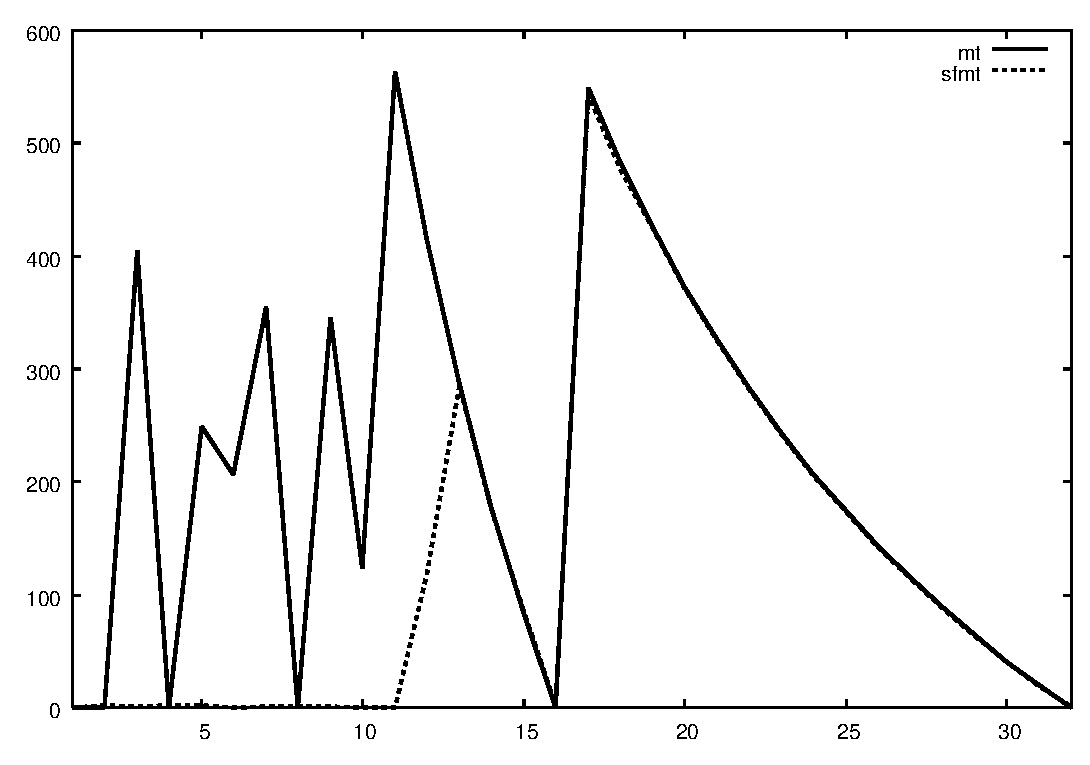
\includegraphics[width=0.8\linewidth,height=0.7\textheight,
keepaspectratio]{delta.eps}
\end{center}
\caption{The dimension defects $d(v)$ of MT (real line) and SFMT (dotted)
for $v=1,2,\ldots, 32$.}
\end{figure}

We also computed the dimension defects of SFMT19937 as a 64-bit
(128-bit) integer generator, and the total dimension 
defect $\Delta$ is 14089 (28676, respectively). In some applications, 
the distribution of LSBs are important. 
To check them, we inverted the order of the bits (i.e. the $i$-th
bit is exchanged with the $(w-i)$-th bit) in each integer, 
and computed the total dimension defect. It is
10328 (21337, 34577, respectively) as
a 32-bit (64-bit, 128-bit, respectively) integer generator.
Throughout the experiments, $d(v)$ is very small for $v\leq 10$.
We consider that these values are satisfactorily small, since
they are comparable with MT
for which no statistical problem 
related to the dimension defect has been reported, 
as far as we know.

\section{Recovery from the 0-excess states}
LFSR with a sparse feedback function $g$ has
the following phenomenon: 
if the bits in the state space 
contain too many 0's and few 1's (called a 0-excess state), then
this tendency continues after considerable generations,
since only small part is changed in the state array
at one generation, and the change is not well-reflected to 
the next generation because of the sparseness.

We measure the recovery time from 0-excess states, 
by the method introduced in \cite{WELL}, as follows.
\begin{enumerate}
\item Choose an initial state with only one bit being 1.
\item Generate $k$ pseudorandom numbers, and discard them.
\item Compute the ratio of 1's among the 
next 32000 bits of outputs
(i.e., in the next 1000 pseudorandom 32-bit integers).
\item Let $\gamma_k$ be the average of the ratio over
all such initial states.
\end{enumerate}
We draw graphs of these ratio $\gamma_k$ $(1 \leq k \leq 20000)$
in Figure~\ref{fig:zero-recovery}
for the following generators: (1) WELL19937c, 
(2) PMT19937 \cite{PMT}, (3) SFMT19937, and (4) MT19937. 
%For (1), (2), (3) and (3), the chosen 
%initial states are those with only one bit being 1
%and all the rest 0. For (2*), the 32 MSBs in the first 128-bit
%integer in the state array is fixed to the value 
%{\tt 6d736d6d} in the hexadecimal form, and the initial states
%are those with only one bit being 1, except these 32 bits.
%Setting these 32 bits to this value assures that SFMT19937
%has the period being a nonzero multiple of $2^{19937}-1$,
%see \S\ref{sec:period}.
\begin{figure}
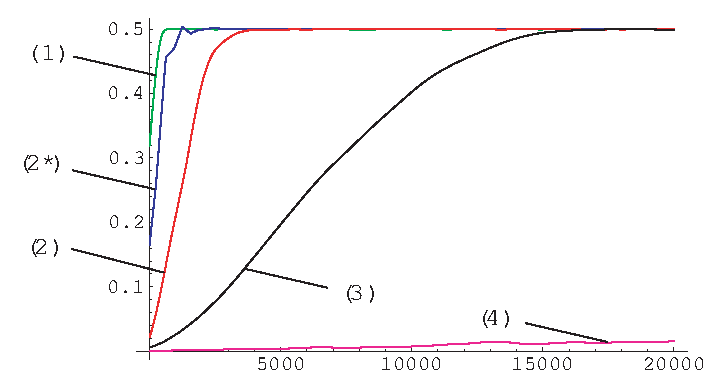
\includegraphics[width=0.7\linewidth]{sfmt.eps}
\caption{$\gamma_k \ (k=0,\ldots,20000)$:
Starting from extreme 0-excess states,
discard the first $k$ outputs and then measure
the ratio $\gamma_k$ of 1's in the next 1000 outputs. 
In the order of the recovery speed: 
(1) WELL19937c, 
(2) PMT19937, (3) SFMT19937, and (3) MT19937.
}\label{fig:zero-recovery}
\end{figure}
Because of its dense feedback, WELL19937c shows
the fastest recovery among the compared. 
SFMT is better than MT, since its recursion refers to 
the previously-computed words (i.e., {\tt W[N-1]} and {\tt W[N-2]}) 
that acquire new 1s, while
MT refers only to the words generated long before 
(i.e., {\tt W[M]} and {\tt W[0]}). PMT19937 shows faster recovery 
than SFMT19937, since PMT19937 has two feedback loops
(hence the name of Pulmonary Mersenne Twister).

The speed of recovery from 0-excess states 
is a trade-off 
with the speed of generation. 
Such 0-excess states will not happen practically, 
since the probability 
that 19937 random bits has less than $19937\times 0.4$ of 1's 
is about $5.7\times 10^{-177}$.
The only the plausible case is that
a poor initialization scheme gives a 0-excess initial state. 
In a typical simulation, the number of 
initializations is far smaller than the number of generations,
therefore we may spend more CPU-time in the initialization
than the generation. Once we avoid the 0-excess initial state
by well-designed initialization, then the recovery 
speed does not matter, in a practical sense. 
Consequently, the slower recovery of SFMT than WELL 
is not an issue, under the assumption that
a good initialization scheme is provided. 

\section{Concluding remarks}
We proposed SFMT pseudorandom number generators, 
which is a very fast generator with satisfactorily
high dimensional equidistribution property. 

\subsection{Trade-off between the speed and the quality}
It is difficult to measure the generation speed of a PRNG in a fair way,
since it heavily depends on the circumstance. 
The 
WELL \cite{WELL} generators have the best possible dimensions of 
equidistribution (i.e. $\Delta=0$)
for various periods ($2^{1024}-1$ to $2^{19937}-1$).
If we use the function call to PRNG
for each generation, then a large part of CPU time
is consumed for handling the function call, and in the 
experiments in \cite{WELL} or \cite{XORSHIFT}, WELL 
is not so slower than MT. On the other hand, if we avoid
the function call, WELL is much slower than MT as seen
in Table~\ref{tab:speed}. 

Since $\Delta=0$, WELL has a better quality than MT or SFMT
in a theoretical sense. 
However, one may argue on whether this difference is 
observable or not. In the case of an $\F2$-linear generator,
the dimension of equidistribution $k(v)$ of $v$-bit accuracy
means that
there is no constant linear relation among the 
$kv$ bits, but there exists a linear relation among
the $(k+1)v$ bits, where $kv$ bits 
($(k+1)v$ bits) are taken from
all the consecutive $k$ integers 
($k+1$ integers, respectively), 
i.e., $v$ MSBs of each of the integers. 
However, the existence of a linear relation does not necessarily
mean the existence of some observable bias.
According to \cite{TESTWEIGHT}, it requires $10^{28}$
samples to detect an $\F2$-linear relation with 
15 (or more) terms among 521 bits, by a standard
statistical test. If the number of the 
total bits is increased, 
the necessary sample size is increased. Thus, it seems
that $k(v)$ of SFMT19937 is sufficiently large, far beyond
the level of the observable bias. 
On the other hand, the speed of the generator is 
observable.
Thus, SFMT focuses more on the speed, for applications
that require fast generations. 

\subsection{Trade-off between the speed and the portability}\label{sec:portability}
There is a trade-off between the speed and the portability.
We prepare (1) a standard C code of SFMT, which uses 
functions specified in C99 only, (2) an optimized C code for
Intel Pentium SSE2, and 
(3) an optimized C code for PowerPC AltiVec. The optimized codes require
icl (Intel C Compiler) or gcc compiler with suitable options.
We will put the newest version of the codes 
in a link from the homepage of \cite{MT}, toghether with some notes 
on compiling with SIMD.

There is a problem of the endian when 128-bit integers 
are converted into 32-bit integers. When a 128-bit integer
is stored as a quadruple of 32-bit integers, in a little
endian system such as Pentium, the 32 MSBs come first.
On the other hand, in a big endian system such as PowerPC,
the 32 LSBs come first. 
The explanation above is based on the former.
To assure the exactly same outputs for both endian systems
as 32-bit integer generators, in the SIMD implementation 
for PowerPC, 
the recursion (\ref{eq:rec-SFMT}) is considered as 
a recursion on quadraples of 32-bit integers, rather than
128-bit integers, so that the content of the state array 
coincides both for little and big endian systems,
as an array of 32-bit integers (not as 128-bit integers).
Then, shift operations on 128-bit integers
in PowerPC differs from those of Pentium. 
Fortunately, 
PowerPC supports arbitrary permutations of 
16 blocks of 8-bit integers in a 128-bit register,
which emulates the Pentium's shift by a multiple of 8.

\appendix
\section{Computation of the Period}\label{sec:period}
%\subsection{Reducible transition function}
LFSR by the recursion (\ref{eq:recursion})
may be considered as an automaton, 
with the state space $S=(\F2^{w})^{N}$
and the state transition function 
$f: S \to S$ given by
$(\bw_0,\ldots,\bw_{N-1})
\mapsto (\bw_1,\ldots,\bw_{N-1}, g(\bw_0,\ldots,\bw_{N-1}))$.  
As a $w$-bit integer generator, the output function is 
$o: S \to \F2^{w},\  (\bw_0,\ldots,\bw_{N-1}) \mapsto \bw_0$.

Let $\chi_f$ be the characteristic polynomial of $f:S \to S$.
If $\chi_f$ is primitive, then the 
period of the state transition takes the maximal value
$2^{\dim(S)}-1$ \cite[\S3.2.2]{knuth:bible}. 
However, to check the primitivity, we need
the integer factorization of this number, which is usually 
impossible for $\dim(S)=nw>10000$. 
On the other hand, the primarity test is much easier than 
the factorization, so many huge primes of the form 
$2^p-1$ are found. 
Such a prime is called a Mersenne prime, and $p$ is
called the Mersenne exponent, which itself is a prime.

MT and WELL discard some fixed $r$-bits from the
array $S$, so that $nw-r$ is a Mersenne exponent. 
Then, the primitivity of $\chi_f$ is easily checked
by the algorithm in \cite[\S3.2.2]{knuth:bible},
avoiding the integer factorization.

SFMT adopted
another method to avoid the integer factorization,
the reducible transition method (RTM), 
which uses a reducible characteristic polynomial.
This idea appeared in \cite{FUSHIMI90}
\cite{BRENT}\cite{BRENT-PRIM}, and 
applications in the present context is 
discussed in detail in another article \cite{PMT}, 
therefore we only briefly recall it. 

Let $p$ be the Mersenne exponent, and $N:=\lceil p/w \rceil$.
Then, we randomly choose parameters for the recursion of LFSR
(\ref{eq:recursion}).
By the Berlekamp-Massey Algorithm, 
we compute the minimal polynomial of the (bit) sequence
generated by the linear recursion. By taking the least
common multiple for several initial values, we have the 
minimal polynomial of the transition $f$. With high 
probability its degree coincides with $\dim(S)$, and if 
this occurs it is the characteristic polynomial $\chi_f$. 
(Note that a direct computation of $\det(tI-f)$ is time-consuming
 because $\dim(S)=19968$.)

By using a sieve, we remove all 
factors of small degree from $\chi_f$,
until we know that it has no irreducible factor of degree $p$,
or we know that it has a factor of degree $p$. 
In the latter case, the factor is 
passed to the primitivity test in \cite[\S3.2.2]{knuth:bible}.

Suppose that we found a recursion with a factor of 
desired degree $p$ in $\chi_f(t)$. Then, 
we have a factorization
$$
\chi_f=\phi_p \phi_r,
$$
where $\phi_p$ is a primitive polynomial of degree $p$
and $\phi_r$ is a polynomial of degree $r=wN-p$. These are coprime, 
if we assume $p>r$.
By linear algebra, we have a decomposition into $f$-invariant subspaces
$$
S=V_p \oplus V_r,
$$
where $f|_{V_p}$ has the minimal polynomial $\phi_p$
and $f|_{V_r}$ has the characteristic polynomial $\phi_r$.
For any element $s \in S$, we denote $s=s_p+s_r$ for the corresponding
decomposition. 

The period length of the state transition is the least common multiple
of that started from $s_p$ and that started from $s_r$. Hence, 
if $s_p \neq 0$, then the period is a nonzero multiple of $2^p-1$. 
By these computation, we checked the following. 
\begin{proposition}
The period of SFMT19937 as 128-bit integer generator is 
a nonzero multiple of $2^{19937}-1$, if the 32 MSBs of 
$\bw_0$ is set to 
the value {\tt 6d736d6d} in the hexadecimal form.
\end{proposition}
The choice of the value for $\bw_0$ is to assure that $s_p\neq 0$.

\begin{remark}
The number of non-zero terms in $\chi_f(t)$ is 
an index measuring the amount of the bit-mixing. 
In the case of SFMT19937, the number of nonzero 
terms is 6711, which is much larger than 135 of MT, 
but smaller than 8585 of WELL19937c. 
\end{remark}

\section{Block-generation}\label{sec:block}
In the block-generation scheme, 
the user of the PRNG specifies an array
of $w$-bit integers of the length $L$, 
where $w=32$, 64 or 128 and $L$ are specified
by the user.
In the case of SFMT19937,
$L$ should be a multiple of $128/w$
and no less than $N \times 128/w$,
since the array needs to accommodate the state space
(note that $N=156$).
By calling the block generation function 
with the pointer to this array, $w$, and $L$, 
the routine fills up the array with
pseudorandom integers, as follows. SFMT19937 keeps the state
space $S$ in an internal array of 128-bit integers of length 156.
We concatenate this state array with the user specified array, 
using the indexing technique.
Then, the routine generates 128-bit integers in the user-specified 
array by the recursion (\ref{eq:rec-SFMT}), as described
in Figure~\ref{fig:B1}, until it fills up the array.
The last 156 128-bit integers
are copied back to the internal array
of SFMT19937. 
This makes the generation much faster than the sequential generation
(i.e., one generation per one call) as shown in Table~\ref{tab:speed}.
\begin{figure}
\begin{center}
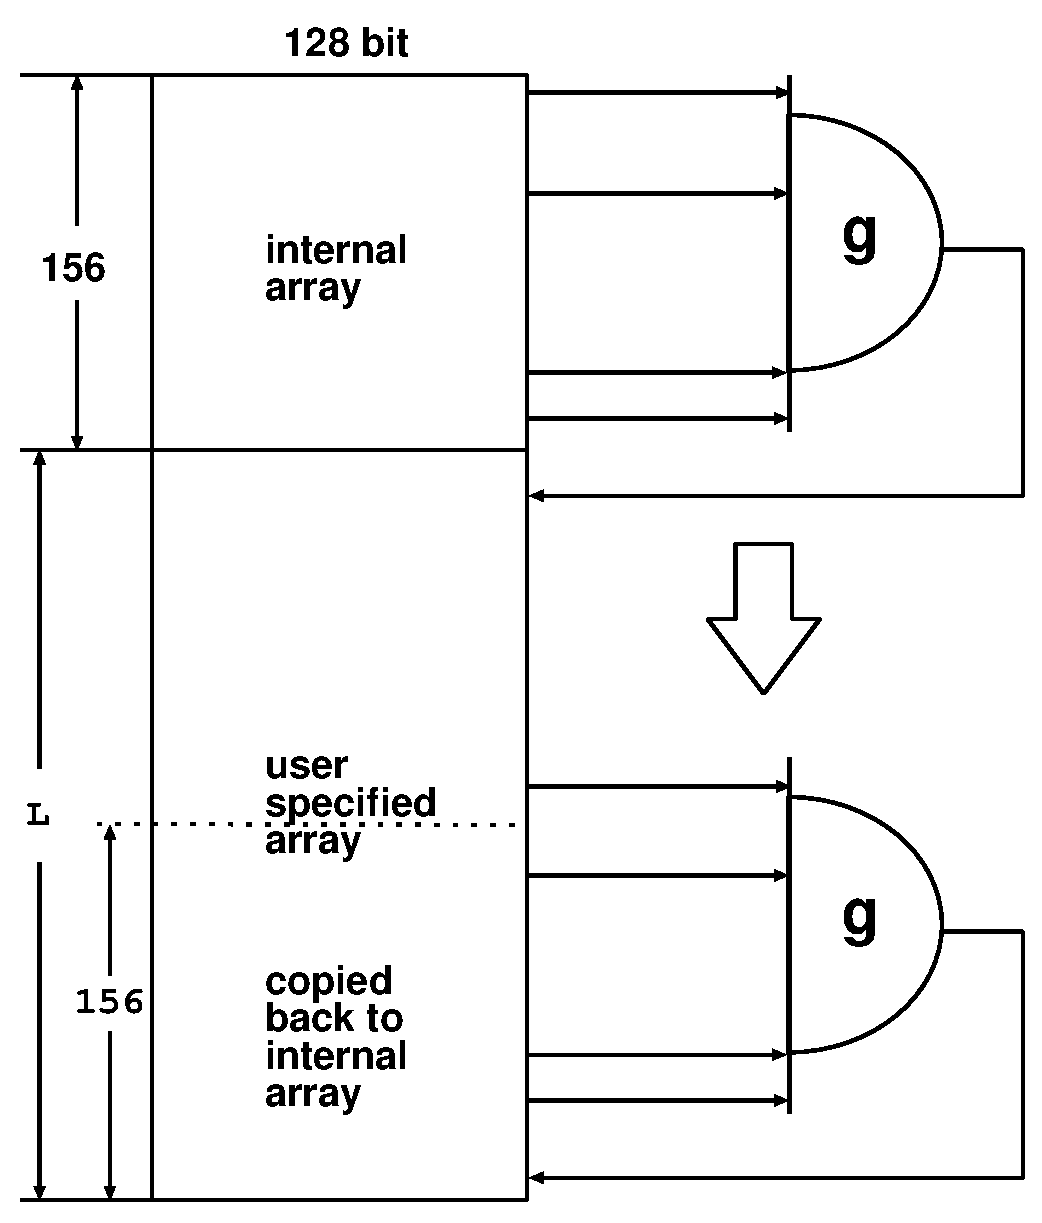
\includegraphics[width=0.7\linewidth,height=0.7\textheight,
keepaspectratio]{fill_array.eps}
\end{center}
\caption{Block-generation scheme}
\label{fig:B1}
\end{figure}

\bibliographystyle{acmtrans}
\bibliography{kuramoto}
\begin{received}
\end{received}
\end{document}
